\documentclass[11pt, oneside]{article} 
\usepackage{geometry}
\geometry{letterpaper} 
\usepackage{graphicx}
	
\usepackage{amssymb}
\usepackage{amsmath}
\usepackage{parskip}
\usepackage{color}
\usepackage{hyperref}

\graphicspath{{/Users/telliott/Github/calculus_book/png/}}
% \begin{center} 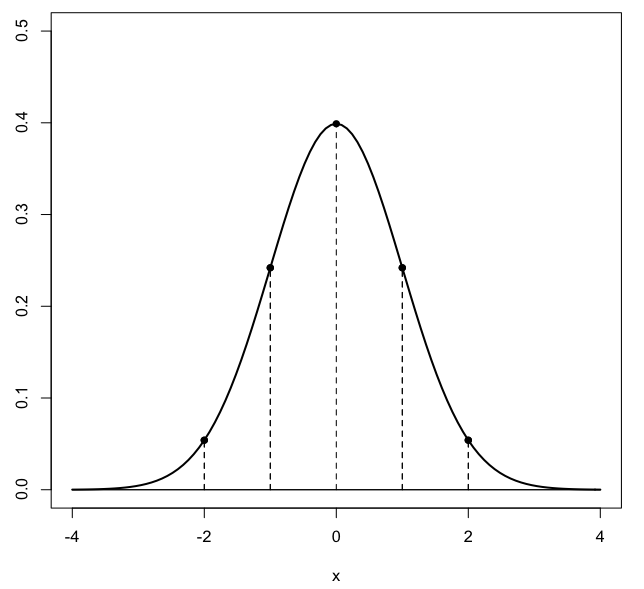
\includegraphics [scale=0.4] {gauss3.png} \end{center}

\title{Basic geometry and congruence of triangles}
\date{}

\begin{document}
\maketitle
\Large

\subsection*{Congruence and similarity of triangles}

$\circ$  Two triangles are \emph{congruent} if and only if they have the same three side lengths.  This is often abbreviated SSS (side-side-side).  

By this definition, a triangle and its mirror image are congruent.  The three triangles shown below are all congruent, even though the first is flipped (it is the mirror image of the other two).

\begin{center} 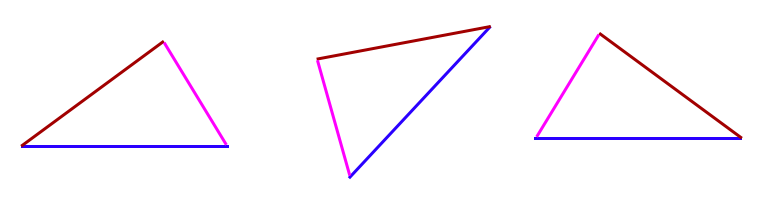
\includegraphics [scale=0.4] {congruent.png} \end{center}

Having the same three sides means that the shape is the same, and all three angles are the same --- the shapes are superimposable, with the proviso that we allow the shape to be flipped over.

In this figure the two smaller triangles obtained by dividing an equilateral triangle in half, are congruent.
\begin{center} 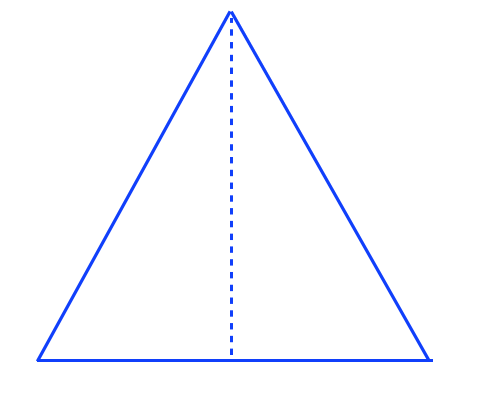
\includegraphics [scale=0.3] {congruent2.png} \end{center}

Some triangles are \emph{similar} but not congruent, with all three angles the same but of different overall sizes.  We could call this AAA (angle-angle-angle).  For similar triangles, the three corresponding pairs of sides are in the same proportions, but re-scaled by the same constant of proportion.

$\circ$  Two triangles are similar if they have the same three angles. 

Because of the angle sum theorem, if any two angles of a pair of triangles are known to be equal, then the third one must be equal as well.

Similar triangles have their sides in the same proportions.

\begin{center} 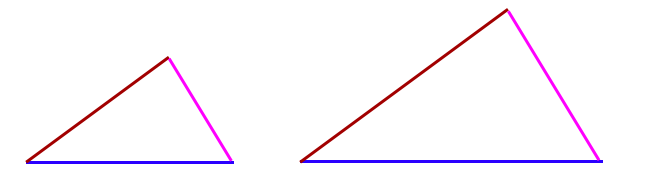
\includegraphics [scale=0.4] {similar.png} \end{center}

Given any triangle, draw a line parallel to one side, which also joins the other two sides.  The new triangle with that side as its base is similar to the given triangle.  Similarity means that all the angles are equal.  This is easily proved using the theorem on alternate interior angles.

\begin{center} 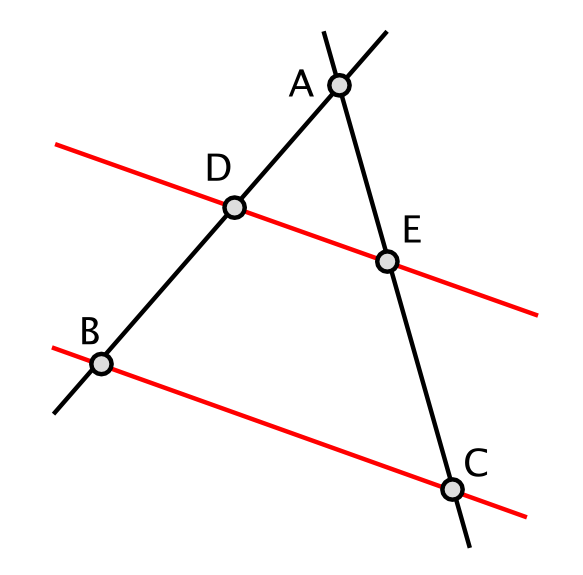
\includegraphics [scale=0.25] {Thales_theorem_1.png} \end{center}
%\begin{center} 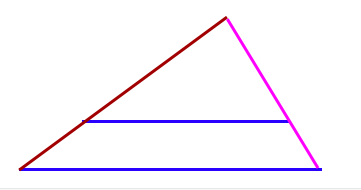
\includegraphics [scale=0.4] {parallel_line.png} \end{center}

In this example, these ratios are all equal
\[ \frac{AD}{AB} = \frac{AE}{AC} = \frac{DE}{BC}  \]

In addition to SSS (side-side-side), there are other conditions that lead to congruence of two triangles when they are satisfied, namely

$\circ$  SAS (side-angle-side)

$\circ$  ASA (angle-side-angle)

$\circ$  AAS (angle-angle-side)

\subsection*{constructions}

Again, the way I think about these conditions is to imagine trying to construct a triangle from the given information, and ask whether it is uniquely determined.  Suppose we know ASA.  The situation is thus:

\begin{center} 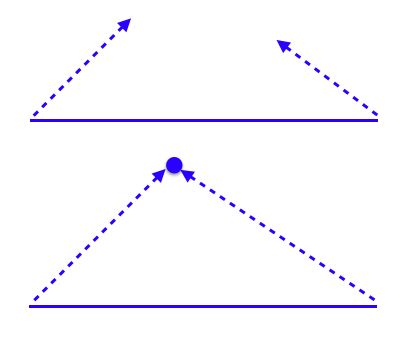
\includegraphics [scale=0.4] {ASA.png} \end{center}
 
Plot the known side and start two other sides from the ends of that side containing the known angles.  They must cross at a unique point.  

But... actually, if we start the two lines pointing below the horizontal, there is another solution, the mirror image.  This triangle is also congruent to the one above.
 
\begin{center} 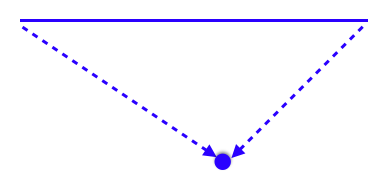
\includegraphics [scale=0.4] {ASA2.png} \end{center}

Alternatively, knowing two angles means we also know the third, because they must add to 180 degrees.  For this reason, ASA and AAS imply that we have exactly the same information, because we know all three angles and (this part is important) we also know \emph{which} two angles flank the known side.
 
For a right-triangle, if the hypotenuse and one leg are equal, the two triangles are congruent.

\begin{center} 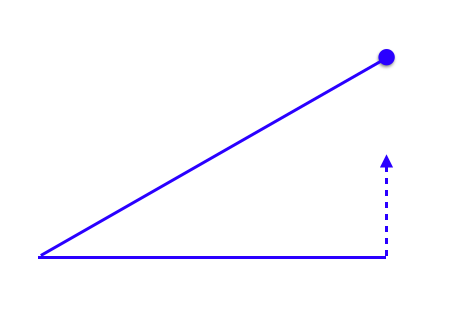
\includegraphics [scale=0.4] {hyp_side_congruent.png} \end{center}

In the figure, imagine the hypotenuse swinging on the hinge of its vertex with the horizontal base.  There is only one angle where it will terminate on the vertical side with the correct length.  This determines the angle between the known sides, or alternatively, the length of the third side.
 
\subsection*{another theorem from Thales}

$\circ$  The base angles of an isosceles triangle are equal.

\begin{center} 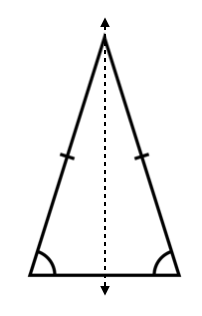
\includegraphics [scale=0.6] {isosceles.png} \end{center}
My favorite proof of this theorem is from symmetry.  Draw a line from the vertex between the two equal sides to the midpoint of the base opposite.  If you turn the triangle over along this axis, we obtain the same triangle back again.  

Alternatively, just say AAS or use the previous theorem on right triangles.

Euclid's proof is here:

\begin{center} 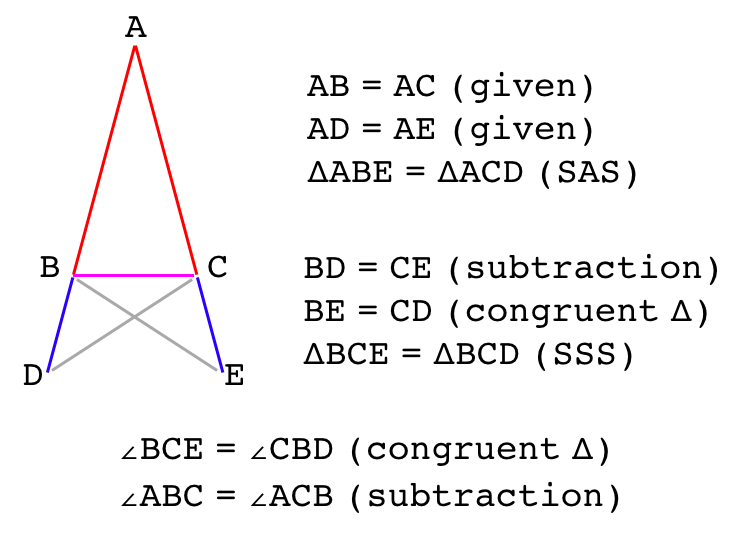
\includegraphics [scale=0.4] {isosceles_proof.png} \end{center}

\subsection*{pyramid height}
As we said, Thales was from Miletus and he lived around 600 BC.  Thales is believed to have traveled extensively around the Mediterranean and was probably of Phoenician heritage, famous sailors.  

During his travels, he went to Egypt, home to the great pyramids at Giza, which were already ancient then.  They were built just around around 2560 BC (dated by reference to Egyptian kings) and were already 2000 years old at that time!

The story is that Thales asked the Egyptian priests about the height of the Great Pyramid of Cheops, and they would not tell him.  So he set about measuring it himself.  The current height is 480 feet.  He used similar triangles.

\begin{center} 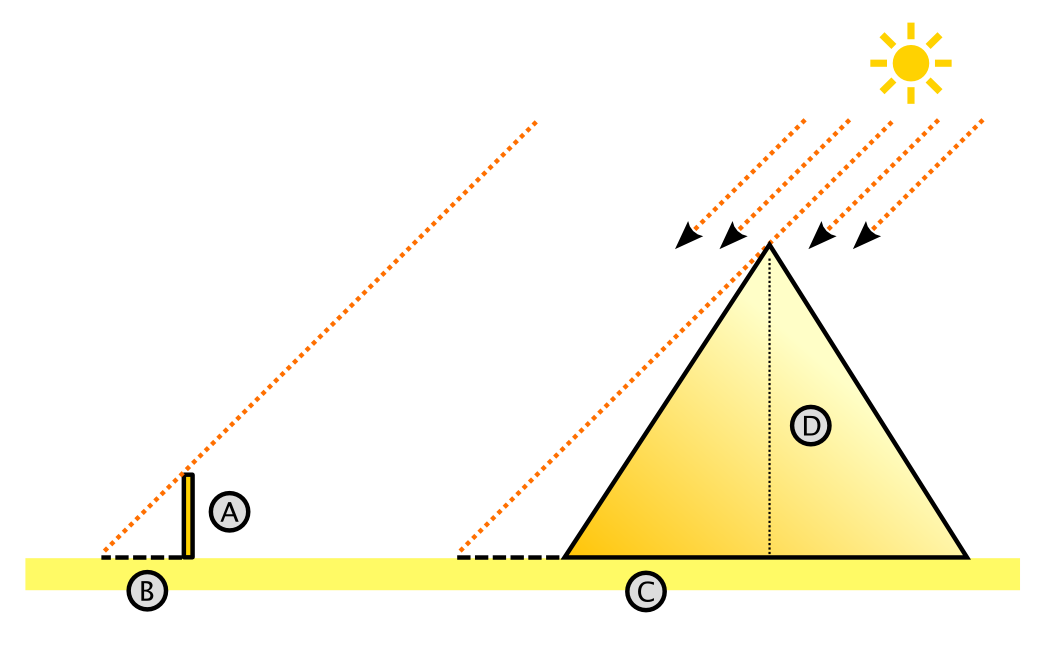
\includegraphics [scale=0.25] {Thales_theorem_6.png} \end{center}

\subsection*{platonic solids}

\url{https://en.wikipedia.org/wiki/Platonic_solid}

\begin{quote}
In three-dimensional space, a Platonic solid is a regular, convex polyhedron. It is constructed by congruent (identical in shape and size) regular (all angles equal and all sides equal) polygonal faces with the same number of faces meeting at each vertex. Five solids meet these criteria.
\end{quote}

\begin{center} 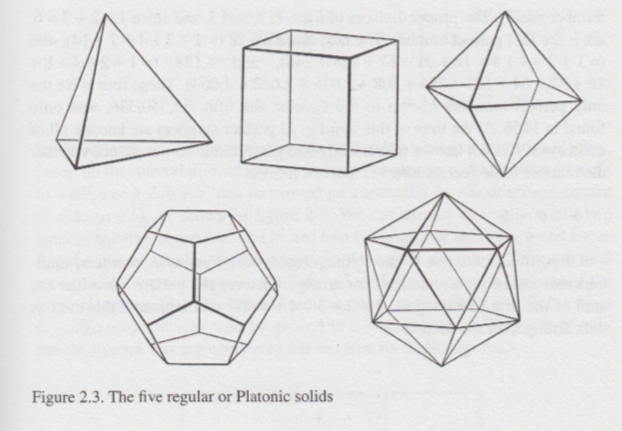
\includegraphics [scale=0.5] {platonic_solids.png} \end{center}
These are:  (i) tetrahedron, (ii) cube, (iii) octagon, (iv) dodecagon, and (v) icosahedron.

There is a wonderful, simple proof that there are only five of them.  Any solid requires at least three sides meeting at each vertex, otherwise the joint between two sides can just flap, like a hinge.  Furthermore, the total of all the vertex angles added up must be less than $360$ degrees, since otherwise the figure would be planar, not 3-dimensional.

So, three equilateral triangles total $60 \times 3 = 180$, four total $60 \times 4 = 240$ and five total $60 \times 5 = 300$.  Six would be a hexagon lying in the plane.  Three squares total $90 \times 3 = 270$, while four give a square array in the plane.  Finally, three pentagons give $108 \times 3 = 324$.  And that's it.  Three hexagons would give $120 \times 3 = 360$, which gives an array in the plane.

Proving that all the angles and side lengths come out correctly, so that the possible solids actually can be constructed is another matter, however.  Euclid devotes book XIII of \emph{The Elements} to this:

\url{https://mathcs.clarku.edu/~djoyce/elements/bookXIII/bookXIII.html#props}


\end{document}